% begin module derivatives-as-function-ex2
\begin{frame}
\begin{example}[Example 2, p. 124]
If $f(x) = x^3-x$, find the formula for $f'(x)$.
\begin{columns}[c]
\column{.25\textwidth}
\ 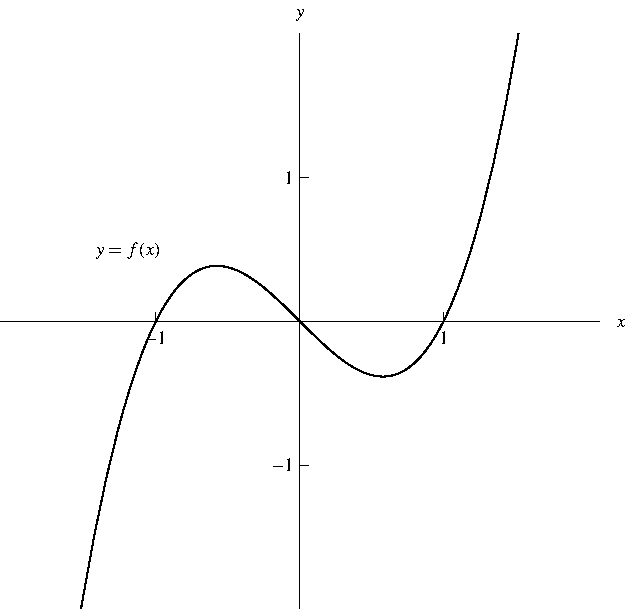
\includegraphics[height=3cm]{derivatives/pictures/03-02-ex2a.pdf}%

\ \only<handout:0| -7>{%
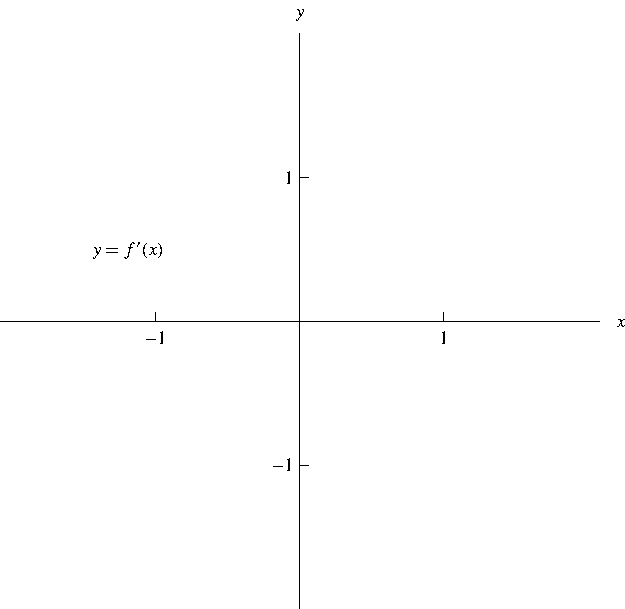
\includegraphics[height=3cm]{derivatives/pictures/03-02-ex2b.pdf}%
}%
\only<8->{%
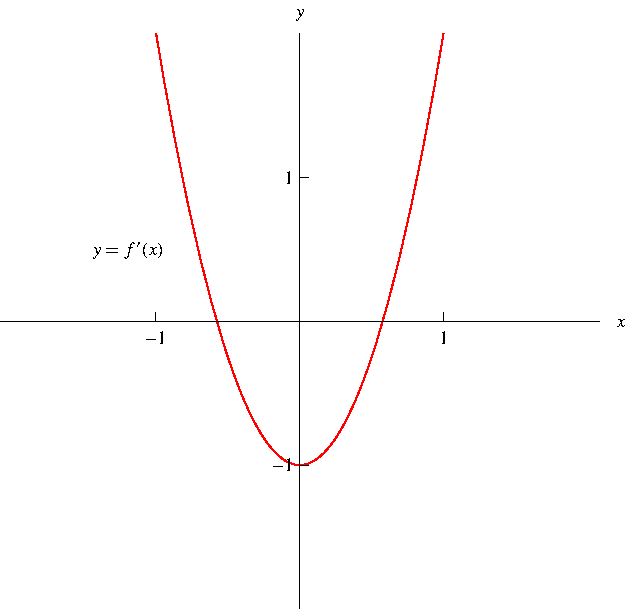
\includegraphics[height=3cm]{derivatives/pictures/03-02-ex2c.pdf}%
}%
\column{.75\textwidth}
\begin{eqnarray*}
&&\uncover<2->{f'(x)}\\%
 & \uncover<2->{ = } &%
\uncover<2->{\lim_{h\rightarrow 0} \frac{f(x+h)-f(x)}{h}}\\%
 & \uncover<3->{ = } &%
\uncover<3->{\lim_{h\rightarrow 0} \frac{[(x+h)^3 - (x+h)]-[x^3-x]}{h}}\\%
 & \uncover<4->{ = } &%
\uncover<4->{\lim_{h\rightarrow 0} \frac{x^3 + 3x^2h+3xh^2+h^3-x-h-x^3+x}{h}}\\%
 & \uncover<5->{ = } &%
\uncover<5->{\lim_{h\rightarrow 0} \frac{3x^2h+3xh^2+h^3-h}{h}}\\%
 & \uncover<6->{ = } &%
\uncover<6->{\lim_{h\rightarrow 0} (3x^2+3xh+h^2-1)}\\%
 & \uncover<7->{ = } &%
\uncover<7->{3x^2-1}\\%
\end{eqnarray*}
\end{columns}
\end{example}
\end{frame}
% end module derivatives-as-function-ex2
